%=============================================================================
% P7 - Ingenius. Manuscrito maquetado en la plantilla oficial de la revista.
%
% Compilar:  pdflatex articulo_p7 && bibtex articulo_p7 && pdflatex articulo_p7 x2
%
% NOTAS DE MAQUETACION
% - El articulo esta escrito en INGLES. Las normas piden el titulo en el idioma
%   del articulo en la primera linea y la traduccion en la segunda. En la clase,
%   \titulo se imprime primero y \tituloa despues, de modo que aqui \titulo
%   lleva el INGLES y \tituloa el ESPANOL. Lo mismo con el resumen: Abstract a
%   la izquierda, Resumen a la derecha.
% - Las palabras clave van en ORDEN ALFABETICO, como pide la plantilla.
% - Las tablas llevan el titulo ARRIBA (\captionof antes del tabular).
% - ANONIMIZADO para revision doble ciego: sin nombres, adscripciones ni ORCID.
%   Rellenar \autores y \adscripcionautor solo en la version no anonima.
%=============================================================================
\documentclass[12pt,twoside,titlepage]{ingenius}
\usepackage[figuresright]{rotating}
\usepackage{pgfplots}
\pgfplotsset{compat=1.7}
\usepackage{adjustbox}
\usepackage{units}
\usepackage{dblfloatfix}
\usepackage{amssymb}
\usepackage{caption}
\usepackage{subcaption}
\usepackage{bm}
\usepackage{textcomp}
\usepackage{pifont}
\usepackage{cite}
\usepackage{xcolor,colortbl}
\usepackage{amsmath}
\usepackage{upgreek}
\usepackage{graphicx}
\usepackage{tikz}
\usetikzlibrary{shapes,arrows}
\usepackage{multirow}
\usepackage{float}
\usepackage{soul}
\usepackage{rotating}
\usepackage{hyperref}
\usepackage{booktabs}
\graphicspath{{figures/}}

%========================================================
% Titulo: ingles primero (idioma del articulo), espanol despues.
\titulo{Signal representation and load transfer in bearing fault
classification: a record-level evaluation on the CWRU dataset}
\tituloa{Representación de señal y transferencia entre cargas en la
clasificación de fallas en rodamientos: una evaluación por registro sobre el
conjunto CWRU}
%========================================================
% VERSION ANONIMIZADA PARA REVISION DOBLE CIEGO.
\autores{}
\adscripcionautor{}

\newcommand{\apellido}{Anonymous et al.}
\newcommand{\titu}{Signal representation and load transfer in bearing fault classification}
\newcommand{\tipo}{Art\'iculo Cient\'if{}ico / Scientif{}ic Paper}
\newcommand{\autor}{}
\newcommand{\pc}{}
\newcommand{\kw}{}
\usepackage{xcolor}
\usepackage{color}
\input{configuracion_paquetes}

\newenvironment{tabla}
  {\par\bigskip\noindent\minipage{\linewidth}}
  {\endminipage\par\bigskip}
\newenvironment{figura}
  {\par\bigskip\noindent\minipage{\linewidth}}
  {\endminipage\par\bigskip}
%========================================================
\begin{document}
\setcounter{page}{1}
% Etiquetas en INGLES, no en espanol como trae la plantilla.
%
% `plantilla_ingenius.tex` (lineas 143-144) y `ingenius.cls` (linea 33, opcion
% `tablename=Tabla` del paquete caption) fijan las etiquetas en espanol, y de
% ahi salian copiadas. Pero la plantilla esta escrita en espanol porque el
% ejemplo lo esta, no porque la revista lo imponga: comprobado el 03/09 sobre
% un articulo en ingles publicado por la propia Ingenius, Contreras Urgiles et
% al. (n.o 21, 2019, DOI 10.17163/ings.n21.2019.03), que es ademas la cita [9]
% de este manuscrito. Sus pies dicen "Figure 1." y "Table 1.", y su
% bibliografia se titula "References".
%
% Antes quedaba una mezcla dentro de la misma frase: el cuerpo decia
% "Table 2 summarises the four" y el pie de esa tabla decia "Tabla 2".
\renewcommand{\refname}{References}
\renewcommand{\figurename}{Figure}
\renewcommand{\tablename}{Table}
\frenchspacing

\begin{tikzpicture}[overlay]
  \node at (138.5mm,12.2mm){
\includegraphics[scale=0.35]{figures/logoingenius.pdf}};
  \node at (138mm,2mm){\textsf{\scriptsize pISSN: 1390-650X / eISSN: 1390-860X}};
  \node at (79mm,10mm){
\includegraphics[scale=0.6]{figures/creativec.pdf}};
\end{tikzpicture}

\input{silabeo}
\membrete
\input{configuracion_portada}

\begin{textblock}{12.4}(0,10)
\adscripcion
\end{textblock}
%========================================================
\begin{table}[htb]
\begin{tabular}{p{8cm}p{8cm}}
{\Large \bfseries Abstract} &{\Large \bfseries Resumen} \\ \\
Comparisons of signal representations for bearing fault diagnosis are usually
reported under a single operating condition, where accuracy saturates and the
comparison carries little information. This work measures how four
representations behave when the test load differs from the training load.
Time-domain statistics, FFT magnitude, db4 wavelet band energies and STFT
spectrogram were combined with three vector classifiers over the sixteen
(training load, test load) pairs of the CWRU drive-end dataset at 12 kHz, with
five folds per cell and a fixed seed. The split was performed by source record
and by purged contiguous blocks, so that no two windows sharing samples fall on
opposite sides. Within a single load, where the split shares records,
all four exceeded 0.95 macro-F1, so the
usual comparison does not discriminate between them. Across loads the mean drop
ranged from 0.074 for the spectrogram to 0.153 for time-domain statistics, with
overlapping bootstrap intervals. The
omnibus Friedman test over the twelve off-diagonal pairs did not reject, while
the three per-classifier tests each did and disagreed on the ranking. An
exploratory three-way ANOVA on the cell means places the representation by
classifier interaction above every main effect. An amplitude-normalisation
ablation did not improve transfer and degraded it with Random Forest. Representation choice interacts with the classifier rather
than defining a general ordering.
&
Las comparaciones entre representaciones de señal para el diagnóstico de fallas
en rodamientos suelen reportarse bajo una sola condición de operación, donde la
exactitud satura y aporta poca información. Este trabajo mide el
comportamiento de cuatro representaciones cuando la carga de prueba difiere de
la de entrenamiento. Se combinaron estadísticos temporales, magnitud FFT,
energías de banda wavelet db4 y espectrograma STFT con tres clasificadores de
vector sobre los dieciséis pares (carga de entrenamiento, carga de prueba) del
conjunto CWRU a 12 kHz, con cinco pliegues por celda y semilla fija. La división
se hizo por registro de origen y por bloques contiguos purgados, evitando fuga
por solape. Dentro de una misma carga, donde la partición comparte
registros, las cuatro superaron 0,95 de F1-macro,
de modo que la comparación habitual no discrimina. Entre cargas la caída media
osciló entre 0,074 para el espectrograma y 0,153 para los estadísticos, con
intervalos de confianza solapados. La prueba de Friedman ómnibus sobre los doce
pares fuera de la diagonal no rechazó, mientras que las tres pruebas por
clasificador rechazaron y discreparon en el orden. Un ANOVA exploratorio sitúa
la interacción representación-clasificador por encima de todo efecto
principal. Una
ablación de normalización de amplitud no mejoró la
transferencia y la degradó con Random Forest. La elección de representación
interactúa con el clasificador.
\\[-0.3cm]
\keywords{bearing fault diagnosis, data leakage, domain shift, Friedman test,
signal representation, vibration analysis}
&
\palabrasclave{análisis de vibraciones, desplazamiento de dominio, diagnóstico
de fallas en rodamientos, fuga de datos, prueba de Friedman, representación de
señal}
\\
\end{tabular}
\end{table}

\newpage

\begin{multicols}{2}
\raggedcolumns
% Sin esto, multicols intenta igualar la altura de las dos columnas
% estirando el espacio elastico de las cabeceras de seccion (\subsection lleva
% "plus" en su salto), lo que produce huecos grandes justo despues de 2.2, 2.5,
% 3.3 y otras subsecciones. \raggedcolumns deja el pie de columna irregular en
% vez de forzar ese estiramiento. Detectado visualmente en el PDF: hay que
% revisar siempre el render, "cero Overfull" no basta.
%========================================================
\section{Introduction}

Rolling element bearings fail in ways that leave a signature in the vibration
measured on the housing. A localised defect produces an impact each time a
rolling element passes over it, and those impacts excite the structural
resonance of the assembly at a repetition rate set by the geometry and the shaft
speed, which is the basis of envelope analysis and of the diagnostic techniques
reviewed in \cite{randall2011}.

Data-driven diagnosis adds a decision on top of that physics: the signal is
converted into some representation and a classifier is trained on it. The choice
of representation is normally justified by comparing several candidates on the
same data and recommending the most accurate. The dataset of the Case Western
Reserve University Bearing Data Center \cite{cwru} is the standard reference for
those experiments, to the point that a benchmark study was devoted to
categorising it and recommending how it should be used \cite{smith2015}, with
later work proposing further improvements to that practice \cite{hendriks2022}.

Accuracy within a single
operating condition saturates near unity, so the ranking it produces separates
methods by hundredths of a point and does not survive a change of dataset. And
the way the data are partitioned decides the result: bearing vibration is
usually cut into overlapping windows, and if those windows are shuffled before
splitting, windows sharing samples end up on both sides and the classifier
recognises the recording rather than the fault. A survey across seventeen
scientific fields found leakage of this kind in 294 papers, in some cases
producing conclusions far more optimistic than the data supported
\cite{kapoor2023}.

The shift between operating conditions is itself an active subject. A review of
deep-learning work on the CWRU dataset records how widely it serves as a
validation reference \cite{neupane2020}, and a benchmark of four architectures
over nine datasets reports generalisation as an open problem of the field
\cite{zhao2020}. The usual response is a domain-adaptation model that aligns the
distributions of a labelled source condition and an unlabelled target condition,
for instance by minimising a multi-kernel maximum mean discrepancy across
several layers \cite{li2019}. That line fixes a representation and modifies the
model, leaving open what the representation itself contributes to the transfer,
which is the question addressed here.

Fault diagnosis in rotating machinery has been addressed repeatedly in this
journal, from measurement rather than from model design. Time-domain descriptors
such as RMS, energy and entropy have been fed to a feed-forward network to
diagnose mechanical faults in spark-ignition engines \cite{contreras2019}, while
temperature and injection pressure have served as measured indicators instead of
a signal representation, with a multifactorial ANOVA establishing which factors
matter \cite{llanes2019}. Earlier, two measurement methods for stator lamination
faults were compared on rotating machines without a learned model
\cite{salazar2012}. The Daubechies db4 wavelet at level four, the family used
for the wavelet representation below, has been applied in the journal to
estimate fault distance \cite{gomez2023}.

This study measures what happens to four representations when the test load
differs from the training load, under a partition designed so that the numbers
are not inflated by overlap. The contributions of this work are: (1) a
record-level evaluation protocol for the CWRU dataset in which the split is
performed by source record and, within a record, by purged contiguous blocks,
verified by a leakage check with a negative control; (2) a 4$\times$4 matrix of
macro-F1 by (training load, test load) pair for four representations and three
classifiers, reported per fold; (3) evidence that no representation holds a
consistent advantage across classifiers, the representation by classifier
interaction being the largest term of the factorial model; and (4) an ablation,
specified in the protocol before the data were split, showing that removing
amplitude information does not improve cross-load transfer.

\section{Materials and Methods}

\subsection{Dataset and label verification}

Forty drive-end accelerometer records of the CWRU Bearing Data Center
\cite{cwru}, sampled at 12 kHz, cover ten class-diameter combinations under four
loads (0, 1, 2 and 3 HP, nominally 1797, 1772, 1750 and 1730 rpm). The classes
are healthy bearing (Normal), inner race fault (IR), ball fault (B) and outer
race fault (OR), the last three at diameters of 0.007, 0.014 and 0.021 inches.

The file naming convention is a known source of error. One file,
\texttt{99.mat} (Normal, 2 HP), holds both \texttt{X098\_DE\_time}, a duplicate of
the 1 HP file, and \texttt{X099\_DE\_time}. Taking the first key ending in
\texttt{\_DE\_time} returns the duplicate and labels the 1 HP signal as 2 HP,
displacing a column of the results matrix with no visible symptom. The channel
is therefore matched exactly against the file number
(\texttt{X\{NNN\}\_DE\_time}), and the script fails rather than falling back to
position.

Labels were verified against the physics of the bearing rather than third-party
tables. For the SKF 6205-2RS JEM drive-end bearing the characteristic order
factors are BPFO 3.5848, BPFI 5.4152, BSF 4.7135 and FTF 0.3983 times the shaft
frequency. Envelope analysis (band-pass filtering in the 2--5.5 kHz resonance,
Hilbert transform, spectrum) confirmed the inner race labels in 12 of 12 records
and the outer race labels in 9 of 12, the expected order dominating by a factor
of three and five. In the healthy records no characteristic frequency stood out,
an order of magnitude below the fault records. Ball faults required the sideband
criterion at twice BSF modulated by FTF, a defective ball striking both races
and crossing the load zone at the cage rate; under it 7 of 12 records exceeded
the healthy baseline. All 40 records were kept, since discarding those with a
weak signature would bias the result upwards, and fault diameter is a covariate
for subgroup reporting.

\subsection{Windowing and the partition rule}

Each record was segmented into windows of 2048 samples with 50 \% overlap,
yielding 5887 windows. The split is performed by source record, never by window,
because overlapping windows of a record share samples.

Outside the diagonal this holds by construction, since training on load $i$ and
testing on load $j$ uses different files; on the diagonal it cannot, because the
dataset provides a single healthy record per load. One rule was therefore
adopted for all sixteen cells: the windows of each record are cut into five
contiguous blocks in time and the first window of each internal block is
discarded. With a stride of 1024 samples and a window of 2048, windows $m$ and
$m+2$ share no samples, so one discarded window per boundary suffices, removing
160 windows (2.7 \%) and leaving 5727. For cell $(i,j)$ and fold $k$, training
uses the blocks other than $k$ from every record of load $i$, and testing block
$k$ from every record of load $j$.

Off the diagonal the rule leaves record-level separation intact and the blocks
only produce five disjoint test sets. On the diagonal, overlap is removed but
training and test windows still come from the same record, so the diagonal is a
reference and is excluded from every test. The training set is four fifths of
one load in all sixteen cells, so no sample-size confound separates the two.

All 80 cell-fold combinations were checked for training windows sharing samples
with a test window of the same record, and none was found. The same check
without the purge reports 320 violations, which is the 160 overlapping pairs
created by four block boundaries in each of the forty records, each counted in
the two folds it affects. Table \ref{tab:ventanas} gives the usable window
counts; the healthy records last 20 to 40 s against about 10 s for the fault
records.

\begin{table}[H]
\centering
\captionof{table}{Usable windows of 2048 samples with 50 \% overlap, by class
and load, after discarding the boundary windows between blocks.}
\label{tab:ventanas}
\begin{tabular}{lrrrr}
\toprule
Class & 0 HP & 1 HP & 2 HP & 3 HP \\
\midrule
Normal & 233 & 467 & 468 & 469 \\
IR     & 340 & 340 & 340 & 342 \\
B      & 341 & 340 & 341 & 341 \\
OR     & 341 & 342 & 340 & 342 \\
\bottomrule
\end{tabular}
\end{table}

\subsection{Signal representations}

Four representations were computed from the same windows. Figure
\ref{fig:senales} shows one raw window per class and Figure \ref{fig:repr} shows
the same inner-race window under the four representations.

\textbf{Time-domain statistics.} The twelve classical vibration descriptors:
mean, RMS, standard deviation, skewness, kurtosis, peak, peak-to-peak, crest
factor, shape factor, impulse factor, clearance factor and mean square root
amplitude.

\textbf{FFT magnitude.} The real FFT magnitude up to Nyquist, 1025 bins of
5.86 Hz.

\textbf{Wavelet db4.} Five-level discrete decomposition with the Daubechies db4
wavelet, the family used in \cite{gomez2023}, as the relative energy of each
band (six values: the approximation A5 and the details D5 to D1).

\textbf{STFT spectrogram.} The spectrogram in dB, normalised per image to
$[0,1]$, with the transform window set explicitly to $\mathit{nperseg} = 64$:
187.5 Hz per band, 63 frames and a hop of 2.67 ms. BPFO and BPFI are not
spectral peaks: the fault excites the 2--5.5 kHz structural resonance and the
characteristic frequency appears as the repetition rate of the impacts, along
the time axis. At 1797 rpm the impacts occur every 9.3 ms (BPFO) and 6.2 ms
(BPFI), so a hop of 2.67 ms places 2.3 to 3.5 frames within each impact period,
while a 512-sample window would give 23.4 Hz per band but a hop of 21.3 ms,
erasing the impact train. For the same reason the spectrogram enters the
comparison as a $16\times64$ grid of 1024 values rather than a square one, which
at that size would leave 10.67 ms per column; the $16\times64$ grid halves the
frequency axis to 375 Hz. A $64\times64$ image of the same transform feeds the
convolutional network.

Table \ref{tab:repr} summarises the four. The scaler is fitted inside the
pipeline, on the training fold only.

\begin{table}[H]
\centering
\captionof{table}{Dimension, effective resolution and dependence on absolute
amplitude of each representation.}
\label{tab:repr}
\resizebox{\columnwidth}{!}{
\begin{tabular}{lrlcc}
\toprule
Representation & Dim. & Effective resolution & Amp.-inv. & In comp. \\
\midrule
Time-domain statistics       & 12   & ---                  & no  & yes \\
FFT magnitude                & 1025 & 5.86 Hz              & no  & yes \\
Wavelet db4 (rel. energy)    & 6    & dyadic band          & yes & yes \\
STFT spectrogram ($16\times64$) & 1024 & 375.0 Hz / 2.67 ms & yes & yes \\
STFT spectrogram ($64\times64$) & 4096 & 187.5 Hz / 2.67 ms & yes & no  \\
\bottomrule
\end{tabular}}
\end{table}

Two of the four discard amplitude by construction, the wavelet returning
relative band energy and the spectrogram being normalised per image, while the
other two keep the absolute scale that varies with load. Comparing them as they
stand would settle any hypothesis about amplitude through the preprocessing
rather than the representation, so an ablation was fixed before results were
examined: time-domain statistics and FFT magnitude recomputed on windows divided
by their RMS value, with SVM-RBF and Random Forest over the twelve off-diagonal
pairs. After normalisation the RMS descriptor equals one in all 5887 windows and
kurtosis is unchanged.

\subsection{Classifiers}

Three classifiers that accept vectors were used with all four representations:
SVM with RBF kernel, Random Forest with 300 trees and a two-layer perceptron of
128 and 64 units trained for at most 500 iterations, all from scikit-learn
\cite{pedregosa2011}. Class weighting was balanced for the SVM and the forest;
the perceptron accepts neither class nor sample weights. A standard scaler was
fitted on the training fold for the SVM and the perceptron, and omitted for the
forest. Hyperparameters were left at the library defaults, so that all four
representations meet each classifier under identical settings. A nested search
on an inner split of the training blocks was possible without touching the test
block; not running one is a limitation, not a constraint of the design.

A two-dimensional convolutional network provides a reference row: three blocks
of 32, 64 and 128 channels with batch normalisation and max pooling, then global
average pooling and a linear layer, in PyTorch \cite{paszke2019}, trained on
$64\times64$ spectrograms for a fixed 30 epochs with Adam at $10^{-3}$ and a
batch of 64. The epoch count is fixed rather than set by early stopping, since a
validation set would either shrink the training set relative to the other
classifiers or select on the test block. The network appears in Table
\ref{tab:f1} but takes no part in the statistical comparison: it has no
counterpart for the other three representations, and an unbalanced design
invalidates both Friedman and the ANOVA.

\subsection{Experimental design and statistical analysis}

The design covers 4 representations $\times$ 3 vector classifiers $\times$ 16
cells $\times$ 5 folds, that is 960 fits, plus 80 for the convolutional
reference and 240 for the ablation. The seed was fixed at 42 and results stored
per fold. The network ran on an RTX 4050 laptop GPU and the rest on CPU.

The statistical procedure was decided before results were examined, following \cite{demsar2006}. The primary test is a Friedman test
over the four representations with the twelve off-diagonal pairs as blocks
($N = 12$, $k = 4$), using macro-F1 averaged over the three classifiers and the
five folds, with a Nemenyi post-hoc test and a critical difference diagram.
The three classifiers share the partition and the signal, so treating each
(pair, classifier) combination as an independent block would raise $N$ to 48 and
halve the critical distance to about 0.68 on the strength of that dependence. As a robustness check a separate Friedman test was
run per classifier, again with $N = 12$, at a Bonferroni-corrected $\alpha = 0.0167$.

A two-way ANOVA on macro-F1 examines representation and load distance (1, 2 or
3 HP of separation; distance 0 is the diagonal and is excluded) with their
interaction, over 240 observations, reporting partial eta squared as the effect
size. Two exploratory departures accompany it. Those 240 observations are 5
folds within each of 48 cells, and folds of one cell share four fifths of their
training windows, so the model was refitted on the 48 cell means. It also
averages over the classifier and so cannot test any term involving it, which a
three-way model on the 144 (representation, classifier, pair) cell means
supplies. The
ablation is reported as a paired difference with a bootstrap confidence interval
and Cliff's delta, since only two conditions are compared.

\begin{figure}[H]
\begin{center}
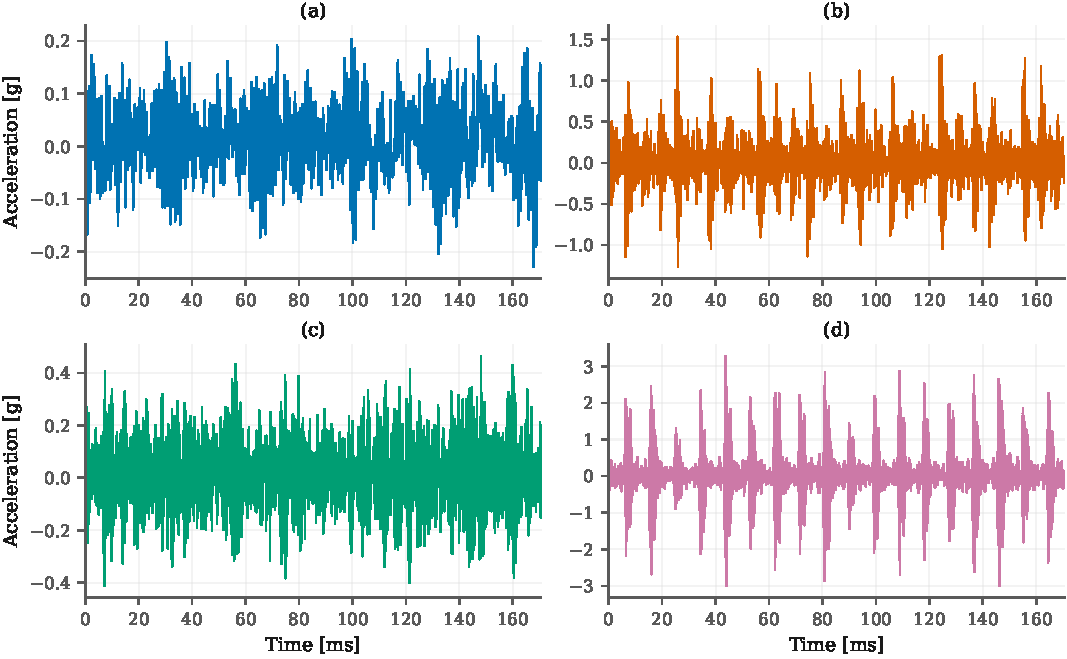
\includegraphics[width=8.17cm]{figures/fig1_p7.pdf}
\end{center}
\caption{Raw drive-end acceleration signals at 0 HP, one 2048-sample window per
class. (a) Normal, (b) inner race, (c) ball, (d) outer race. Each panel has its
own $y$-axis scale: record RMS ranges from 0.066 g (Normal) to 0.425 g (outer
race), so a shared scale would flatten three panels.}
\label{fig:senales}
\end{figure}

\begin{figure}[H]
\begin{center}
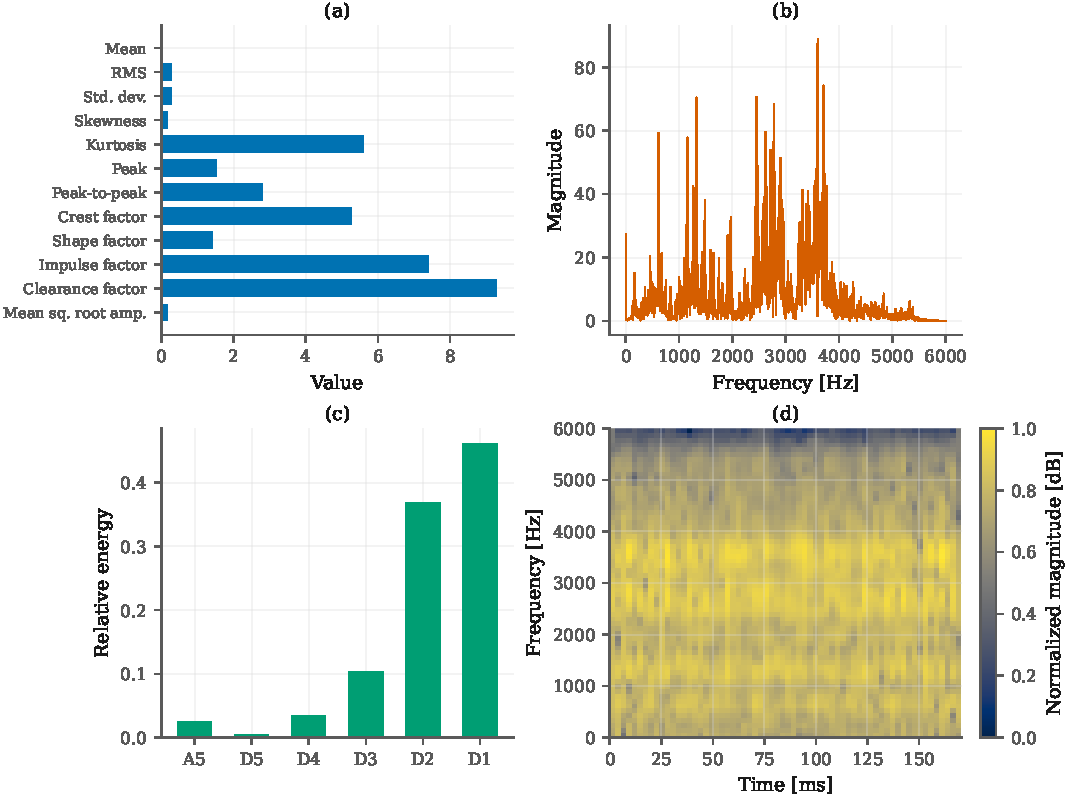
\includegraphics[width=8.17cm]{figures/fig2_p7.pdf}
\end{center}
\caption{Same inner-race fault window at 0 HP under the four representations.
(a) Time-domain statistics, (b) FFT magnitude, (c) db4 wavelet relative energy
per band, (d) STFT spectrogram on the $64\times64$ CNN grid, not the
$16\times64$ grid that enters the comparison. The twelve descriptors of (a) do
not share units; wavelet bands run from coarsest approximation (A5) to finest
detail (D1).}
\label{fig:repr}
\end{figure}

\section{Results and Discussion}

\subsection{In-domain performance saturates}

Within a single load all four representations exceed 0.95 macro-F1, averaged
over classifiers: 0.9997 for FFT magnitude, 0.9925 for the spectrogram, 0.9882
for time-domain statistics and 0.9602 for the wavelet, with the breakdown by
classifier in Table \ref{tab:f1}. Under four hundredths separate best from worst
and ten of the twelve representation-classifier combinations sit above 0.98, so
a comparison restricted to the training condition separates little.

\begin{table}[H]
\centering
\captionof{table}{Macro-F1 (mean $\pm$ standard deviation over folds and cells)
in-domain and out-of-domain, by representation and classifier. The convolutional
network is a reference row and takes part in neither Friedman nor the ANOVA.
The best value in each column is in bold, among the twelve rows that enter the
comparison; the in-domain column has two rows tied at 1.000.}
\label{tab:f1}
\resizebox{\columnwidth}{!}{
\begin{tabular}{llcc}
\toprule
Representation & Classifier & F1 in-domain & F1 out-of-domain \\
\midrule
Statistical & MLP           & 0.988 $\pm$ 0.015 & 0.799 $\pm$ 0.229 \\
Statistical & Random Forest & 0.992 $\pm$ 0.008 & 0.869 $\pm$ 0.103 \\
Statistical & SVM-RBF       & 0.985 $\pm$ 0.020 & 0.836 $\pm$ 0.174 \\
FFT & MLP                   & \textbf{1.000 $\pm$ 0.000} & \textbf{0.971 $\pm$ 0.043} \\
FFT & Random Forest         & \textbf{1.000 $\pm$ 0.000} & 0.956 $\pm$ 0.054 \\
FFT & SVM-RBF               & 0.999 $\pm$ 0.003 & 0.774 $\pm$ 0.061 \\
Wavelet db4 & MLP           & 0.969 $\pm$ 0.017 & 0.830 $\pm$ 0.087 \\
Wavelet db4 & Random Forest & 0.982 $\pm$ 0.011 & 0.892 $\pm$ 0.045 \\
Wavelet db4 & SVM-RBF       & 0.929 $\pm$ 0.018 & 0.850 $\pm$ 0.074 \\
STFT spectrogram & MLP           & 0.998 $\pm$ 0.003 & 0.916 $\pm$ 0.056 \\
STFT spectrogram & Random Forest & 0.980 $\pm$ 0.011 & 0.898 $\pm$ 0.069 \\
STFT spectrogram & SVM-RBF       & 0.999 $\pm$ 0.001 & 0.942 $\pm$ 0.054 \\
\midrule
CNN 2D (reference) & CNN2D  & 0.971 $\pm$ 0.116 & 0.957 $\pm$ 0.119 \\
\bottomrule
\end{tabular}}
\end{table}

\subsection{Cross-load degradation}

Figure \ref{fig:mapa} shows macro-F1 for every (training load, test load) pair,
one panel per representation, diagonal boxed. Averaged over the twelve
off-diagonal cells, the drop from the diagonal is 0.074 for the spectrogram,
0.0995 for FFT magnitude, 0.1029 for the wavelet and 0.1534 for time-domain
statistics. Resampling the twelve pairs gives intervals of 0.043--0.105,
0.080--0.122, 0.073--0.133 and 0.074--0.240, which all overlap. The
representation retaining absolute amplitude degrades most, but the attribution
to the time-frequency nature of the representation does not hold, since FFT
magnitude, which carries no time information, degrades slightly less than the
wavelet.

Degradation grows with load distance at different rates: at one step the four
lie between 0.887 and 0.943 and at three steps between 0.655 and 0.880, most of
the widening from time-domain statistics.

The matrix is also asymmetric. With time-domain statistics, training at 0 HP and
testing at 1 HP gives 0.795 against 0.678 for the reverse; at maximum separation
the two directions give 0.771 and 0.539, the worst cell of the matrix. Testing
at 0 HP is the harder direction throughout, and the healthy class has 233
windows at 0 HP against about 468 elsewhere.

The spectrogram is also the most expensive of the four to extract, 5.96 s over
the 5887 windows against 0.27 s for FFT magnitude.

The convolutional reference scores 0.971 in-domain, the lowest of the five rows,
and 0.957 out of domain, the highest, a drop of 0.0135. A training failure
governs both. Trained at 0, 1 and 2 HP it reaches 0.998, 1.000 and 0.992
in-domain, and 0.892 $\pm$ 0.230 at 3 HP; the deficit is one of the five folds
at 3 HP, whose four cells fall between 0.396 and 0.489, consistent with the
network not converging within the fixed 30 epochs. That fold also produces the
standard deviations of 0.116 and 0.119. It is reported as it ran, since the
epoch budget was fixed in advance. The row is descriptive and its apparent
advantage in transfer should not be read as one.

% Fig. 3 es mas ancha que una columna (16 cm) y no cabe a media columna, asi
% que no puede ir con [H] dentro del flujo de multicols como las demas figuras
% y tablas. Como figure*[t] normal, LaTeX la trata como flotante en cola: espera
% el siguiente hueco de pagina completa, que caia DESPUES de donde el texto ya
% habia colocado la Fig. 4 (columna simple, [H]), invirtiendo el orden de
% lectura. Probado \clearpage antes de esta figura: empeora el problema (deja
% una pagina casi vacia y aun asi no garantiza el orden, porque clearpage solo
% termina la pagina, no fuerza que ESTE flotante en particular ocupe la
% siguiente). La solucion correcta es sacarla de multicols: se cierra el
% entorno de dos columnas, se inserta la figura a ancho completo exactamente
% aqui (sin cola de flotantes, sin ambiguedad de orden) y se reabre multicols
% despues. Es la tecnica estandar para figuras anchas dentro de multicols.
\end{multicols}
\begin{figure}[H]
\begin{center}
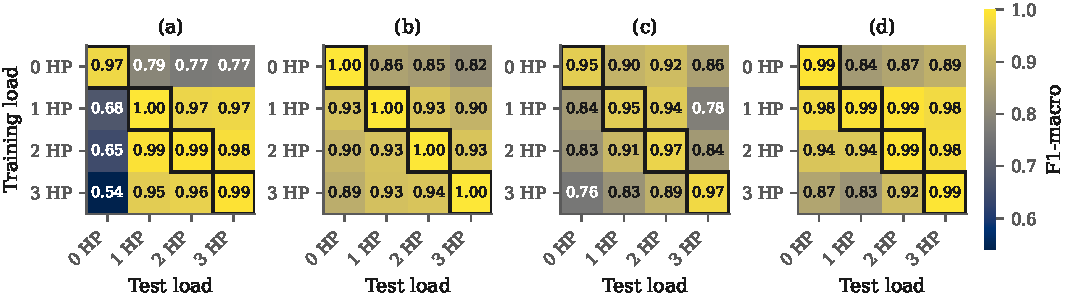
\includegraphics[width=16cm]{figures/fig3_p7.pdf}
\end{center}
\caption{Macro-F1 for every (training load, test load) pair, averaged over the
three vector classifiers and 5 folds. (a) Statistical, (b) FFT, (c) Wavelet db4,
(d) STFT spectrogram. The diagonal is a reference cell, boxed for orientation,
and takes part in neither Friedman nor the ANOVA: with a single Normal recording
per load it does not admit a record-level split.}
\label{fig:mapa}
\end{figure}
\begin{multicols}{2}
\raggedcolumns

\subsection{No consistent ranking across classifiers}

The primary Friedman test over the twelve off-diagonal pairs does not reject:
$\chi^2 = 5.20$, $p = 0.158$, with mean ranks of 1.833 for the spectrogram,
2.500 for FFT magnitude, 2.667 for time-domain statistics and 3.000 for the
wavelet, against a Nemenyi critical distance of 1.354. No pair is separated in
the critical difference diagram of Figure \ref{fig:nemenyi}, the smallest
post-hoc $p$-value being 0.119, between the wavelet and the spectrogram.

The three per-classifier tests each reject and disagree on the ordering. The
spectrogram ranks first with SVM-RBF ($\chi^2 = 17.10$, $p = 0.00067$), where
FFT magnitude ranks last at 3.500; FFT magnitude ranks first with Random Forest
($\chi^2 = 13.70$, $p = 0.0033$, rank 1.333) and with the perceptron
($\chi^2 = 21.00$, $p = 0.00011$, rank 1.083), all three surviving the
Bonferroni-corrected $\alpha = 0.0167$. Averaging them for the primary test
cancels that disagreement, which is why the omnibus test does not reject while
its components do.

The two-way ANOVA of the protocol, over the 240 fold-level observations, returns
representation ($F = 15.93$, $\eta^2_p = 0.173$), load distance ($F = 35.51$,
$\eta^2_p = 0.238$) and their interaction ($F = 5.14$, $\eta^2_p = 0.119$) as
significant at $p < 0.001$ over 228 residual degrees of freedom. Those degrees
of freedom assume independent folds, and consecutive folds share four fifths of
their training windows. Refitting on the 48 cell means removes the assumption
and most of the result: load distance survives ($F = 5.85$, $p = 0.006$),
representation falls to $F = 2.62$, $p = 0.065$, and the representation by
load-distance interaction to $F = 0.85$, $p = 0.543$. That interaction is an
artefact of treating folds as replicates and is not claimed here.

Adding the classifier as a factor locates the effect elsewhere (Table
\ref{tab:anova}). The representation by classifier interaction is the largest
term of the model ($F = 4.91$, $p < 0.001$, $\eta^2_p = 0.214$), above every main
effect, while representation by load distance is not significant ($F = 1.76$,
$p = 0.113$). The effect of representation depends on the classifier, which the
three disagreeing Friedman tests already indicated.

That model treats the twelve pairs as interchangeable replicates within each
level of load distance, and they are not: every load appears in six of them.
Entering the pair as a block absorbs the dependence, at the cost of load
distance, which is a function of the pair and leaves the model. The interaction
survives and grows slightly ($F = 5.78$, $p < 0.001$, $\eta^2_p = 0.223$ over 121
residual degrees of freedom), while the block takes the largest share
($F = 4.87$, $\eta^2_p = 0.307$): which two loads are crossed matters more than
any factor of the design, and load distance does not capture all of it. All
models beyond the one specified in the protocol are exploratory and their
$p$-values are uncorrected.

\begin{table}[H]
\centering
\captionof{table}{Exploratory three-way ANOVA on macro-F1 over the 144
off-diagonal cells, with the five folds of each cell averaged. The diagonal is
excluded and the convolutional network takes no part.}
\label{tab:anova}
\resizebox{\columnwidth}{!}{
\begin{tabular}{lrrrrr}
\toprule
Source & SS & df & $F$ & $p$ & $\eta^2_p$ \\
\midrule
Representation (R)      & 0.1595 & 3   & 5.47  & 0.002    & 0.132 \\
Classifier (C)          & 0.0687 & 2   & 3.53  & 0.033    & 0.061 \\
Load distance (D)       & 0.2370 & 2   & 12.18 & $<0.001$ & 0.184 \\
R $\times$ C            & 0.2865 & 6   & 4.91  & $<0.001$ & 0.214 \\
R $\times$ D            & 0.1030 & 6   & 1.76  & 0.113    & 0.089 \\
C $\times$ D            & 0.0178 & 4   & 0.46  & 0.766    & 0.017 \\
R $\times$ C $\times$ D & 0.0336 & 12  & 0.29  & 0.990    & 0.031 \\
Residual                & 1.0504 & 108 &       &          &       \\
\bottomrule
\end{tabular}}
\end{table}

\begin{figure}[H]
\begin{center}
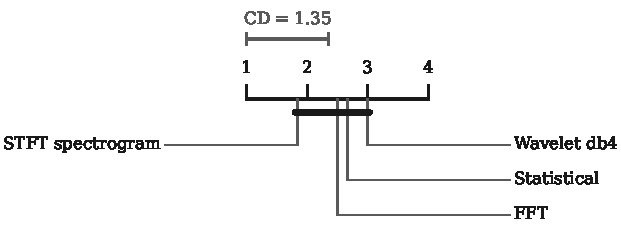
\includegraphics[width=8.17cm]{figures/fig4_p7.pdf}
\end{center}
\caption{Nemenyi critical-difference diagram for the primary Friedman test
($N = 12$ off-diagonal pairs, $k = 4$ representations, $\chi^2 = 5.20$,
$p = 0.158$). Representations joined by a bar are not distinguishable at
$\alpha = 0.05$; CD is the Nemenyi critical distance.}
\label{fig:nemenyi}
\end{figure}

\subsection{Performance by fault diameter}

Over the off-diagonal cells recall is highest for the healthy class (0.994) and
lowest for inner race faults at 0.014 in (0.587). The next four subgroups are
ball at 0.021 in (0.786), inner race at 0.021 in (0.823), inner race at 0.007 in
(0.832) and outer race at 0.014 in (0.849); the remaining four sit above 0.89.
Only the first is separated from the rest by a wide margin.

Envelope verification had already identified two of those subgroups, the outer
race records at 0.014 in and the ball records at 0.021 in, as having a weak
signature. The inner race subgroup at 0.014 in was not, since envelope analysis
confirmed all twelve inner race records. The two ask different questions:
whether the signature is detectable within a record, and whether a classifier
trained on one load recognises it at another. The representations disagree
sharply on it, recall being 0.836 with
FFT magnitude against 0.485 with the spectrogram, 0.494 with time-domain
statistics and 0.533 with the wavelet, so a single subgroup carries part of the
representation by classifier interaction.

\subsection{Amplitude normalisation does not explain the transfer gap}

The ordering in the cross-load results suggests that representations retaining
absolute amplitude degrade because amplitude scales with load. The ablation
tests it by dividing each window by its RMS value before extracting the two
amplitude-dependent representations. No combination improved by an interval that
excludes zero, and two degraded. With Random Forest, time-domain statistics lost 0.149 macro-F1 (95 \% CI
$-0.197$ to $-0.103$, Cliff's delta $-0.472$) and FFT magnitude lost 0.133
(95 \% CI $-0.151$ to $-0.116$, delta $-0.750$). With SVM-RBF both intervals
cross zero: $-0.018$ for statistics (95 \% CI $-0.047$ to $+0.011$) and $+0.033$
for FFT (95 \% CI $-0.002$ to $+0.067$, delta 0.330). That last interval
contains zero, so the ablation separates the two classifiers rather
than ruling out any benefit: normalisation is harmful with the forest and of
uncertain benefit with the SVM.

Removing amplitude therefore does not help transfer with the forest, and the
ordering observed above requires an explanation other than amplitude dependence
alone.

\subsection{Limitations}

Each combination of fault type and diameter in the CWRU dataset is a single
physical bearing measured under four loads, so crossing loads keeps the bearing
fixed and a model may rely on the signature of that specimen rather than on the
fault type. The degradation measured here is therefore a lower bound, and
external validation on another machine is left as future work.

The diagonal cells cannot use a record-level split, since the dataset provides
one healthy record per load. Their purged blocks remove leakage through overlap
but not the correlation of sharing a record; they are excluded from every test
and the in-domain figures of Table \ref{tab:f1} are a reference level, not an
estimate of generalisation. That single healthy record also leaves the class
imbalanced differently across loads, 233 windows at 0 HP against about 468
elsewhere. Macro-F1 and class weighting mitigate this, but the perceptron
accepts no class weights and the direction asymmetry reported above is
consistent with the imbalance being part of the cause rather than an effect of
load alone.

The envelope spectrum, the reference technique of the field and the one used
here to verify the labels, is not among the four representations, which were
fixed before the data were touched. It keeps the impact repetition rate and
discards the carrier, which makes it the likeliest to transfer across loads, so
its absence limits what the comparison covers.

Hyperparameters were left at their defaults, so the per-classifier ranking holds
under those defaults only, and the four representations differ in dimension by
two orders of magnitude, from 6 to 1025. The two interact: an untuned SVM on
1025 FFT bins is a plausible partial explanation for FFT magnitude ranking last
with that classifier and first with the other two. Equalising dimension was
rejected because dimension is part of a representation, and a nested search on
the training blocks would separate the two readings.

The twelve blocks of the Friedman test are not independent. Each load appears in
six pairs, and the pairs $(i,j)$ and $(j,i)$ use the same two sets of records
with the roles exchanged, so the exchangeability the test assumes is violated in
a direction that cannot be signed without a variance component per load. The
blocked ANOVA above measures how much variance the pair carries, but no test
here escapes the dependence and, with four loads, no design on this dataset
would. The $p$-value of 0.158 is a failure to separate the four representations,
not evidence that they are equivalent. For the same reason the results are not
placed beside published cross-load figures, which are reported under partitions
this protocol was designed to avoid: the difference would measure the partition
rather than the method.

\section{Conclusions}

Within a single load the four representations all exceed 0.95 macro-F1 and
separate by less than four hundredths, so a comparison under the training
condition alone does not identify a preferable one. Once the test load differs
the spread widens, from 0.074 for the STFT spectrogram to 0.153 for time-domain
statistics, the latter falling to 0.655 macro-F1 at three steps of separation.
The bootstrap intervals of those four figures overlap, so the ordering they
suggest is not established.

That spread does not translate into a general recommendation. The omnibus
Friedman test over the twelve off-diagonal pairs does not reject
($\chi^2 = 5.20$, $p = 0.158$), the three per-classifier tests each reject and
place a different representation first, and the largest term of the factorial
model is the representation by classifier interaction. FFT magnitude ranks last
with SVM-RBF and first with the other two. Representation and classifier should
therefore be chosen together, since a recommendation drawn from one classifier
does not carry to another.

The mechanism usually offered for the advantage of amplitude-invariant
representations was not supported. RMS normalisation improved cross-load
transfer in none of the four tested combinations by an interval excluding zero,
and degraded it with Random Forest by 0.149 for time-domain statistics and 0.133
for FFT magnitude. On this evidence, removing absolute amplitude does not buy
transfer.

External validation on a different machine would separate the degradation
attributable to load from that masked by reusing one physical bearing per fault
condition. Subgroup reporting would also repay attention: the inner race
subgroup at 0.014 in reached a recall of 0.587 across loads, with the four
representations disagreeing by more than three tenths.

%========================================================
\section*{Data availability}

% Se cita SOLO el DOI de Zenodo, no la URL de GitHub: esa URL contiene el
% usuario del primer autor y desanonimizaria el manuscrito, que va a revision
% doble ciego. El DOI no revela autoria y cumple igual el checklist de la guia.
The CWRU records are public \cite{cwru}. The analysis code, the per-fold results
and the scripts generating every table and figure are deposited with the DOI
10.5281/zenodo.22907922.
%========================================================

\bibliography{referencias.bib}
\bibliographystyle{IEEEtran}
\end{multicols}
\end{document}
